\clearpage

\section{Appendix}\label{sec:appendix}

\begin{table*}[t]
    \centering
    \fontsize{8pt}{7pt}\selectfont
    \setlength{\tabcolsep}{4pt}
    \renewcommand{\arraystretch}{1.4}
    \begin{tabularx}{\linewidth}{rlX}\toprule
        \# & Title & Hypothesis \\\midrule
        1 & Explicit identification & All Confidential Information shall be expressly identified by the Disclosing Party. \\
        2 & Non-inclusion of non-technical information & Confidential Information shall only include technical information. \\
        3 & Inclusion of verbally conveyed information & Confidential Information may include verbally conveyed information. \\
        4 & Limited use & Receiving Party shall not use any Confidential Information for any purpose other than the purposes stated in Agreement. \\
        5 & Sharing with employees & Receiving Party may share some Confidential Information with some of Receiving Party's employees. \\
        6 & Sharing with third-parties & Receiving Party may share some Confidential Information with some third-parties (including consultants, agents and professional advisors). \\
        7 & Notice on compelled disclosure & Receiving Party shall notify Disclosing Party in case Receiving Party is required by law, regulation or judicial process to disclose any Confidential Information. \\
        8 & Confidentiality of Agreement & Receiving Party shall not disclose the fact that Agreement was agreed or negotiated. \\
        9 & No reverse engineering & Receiving Party shall not reverse engineer any objects which embody Disclosing Party's Confidential Information. \\
        10 & Permissible development of similar information & Receiving Party may independently develop information similar to Confidential Information. \\
        11 & Permissible acquirement of similar information & Receiving Party may acquire information similar to Confidential Information from a third party. \\
        12 & No licensing & Agreement shall not grant Receiving Party any right to Confidential Information. \\
        13 & Return of confidential information & Receiving Party shall destroy or return some Confidential Information upon the termination of Agreement. \\
        14 & Permissible copy & Receiving Party may create a copy of some Confidential Information in some circumstances. \\
        15 & No solicitation & Receiving Party shall not solicit some of Disclosing Party's representatives. \\
        16 & Survival of obligations & Some obligations of Agreement may survive termination of Agreement. \\
        17 & Permissible post-agreement possession & Receiving Party may retain some Confidential Information even after the return or destruction of Confidential Information. \\
        \bottomrule
    \end{tabularx}
    \caption{List of hypotheses. The titles are only used for human readabilities.}\label{tab:hypotheses}
\end{table*}


\subsection{Details on Data Collection}\label{sec:appendix-data-collection}

In this section, we provide supplemental information regarding the data collection discussed in \cref{sec:system-data}.

As discussed in \cref{sec:system-formulation}, our dataset consists exclusively of non-disclosure agreements (NDAs) in order to incorporate more fine-grained hypotheses.
More specifically, we used unilateral or bilateral NDAs or confidentiality agreement between two parties.
We excluded employer-employee NDAs and those that are part of larger agreements (such as a confidentiality agreement inside a larger merger agreement), because they are quite different from the rest of NDAs.

We collected NDAs from Internet search engines and Electronic Data Gathering, Analysis, and Retrieval system (EDGAR).
For the collection from the search engines, we queried Google search engines with a search query ``\,``non-disclosure'' agreement filetype:pdf'' and downloaded the PDF files that the search engines returned.
We note that Google search engines in different domains return different results.
Therefore, we used seven domains from countries where English is widely spoken (US ``.com'', UK ``.co.uk'', Australia ``.com.au'', New Zealand ``.co.nz'', Singapore ``.com.sg'', Canada ``.ca'' and South Africa ``.co.za'').
Since collected PDFs contain irrelevant documents, we manually screened all 557 documents and removed all the irrelevant documents.
We also removed NDAs that do not have embedded texts (i.e., glyphs are embedded as an image) or those that have more than one columns, since they are difficult to preprocess.

For the collection from EDGAR, we first download all the filed documents from 1996 to 2020 in a form of daily archives\footnote{\url{https://www.sec.gov/Archives/edgar/Oldloads/}}.
We uncompressed each archive and deserialized files using regular expressions by referencing to the EDGAR specifications \cite{sec_edgar_2018}, which gave us 12,851,835 filings each of which contains multiple documents.
We then extracted NDA candidates by a rule-based filtering.
Using meta-data obtained during the deserialization, we extracted documents whose file type starts with ``EX'' (denotes that it is an exhibit), its file extension is one of ``.pdf'', ``.PDF'', ``.txt'', ``.TXT'', ``.html'', ``.HTML'', ``.htm'' or ``HTM'', and its content is matched by a regular expression ``(?<![a-zA-Z\.,\-"()]\textvisiblespace*)([Nn]on[-\textvisiblespace][Dd]isclosure)|(NON[-\textvisiblespace]DISCLOSURE)''.
We manually screened all 28,780 NDA candidates and obtained 236 NDAs.
All of the NDAs from EDGAR were either in HTML or plain text format.

\begin{figure}[tb]
    \centering
    \begin{subfigure}[b]{0.49\textwidth}
        \centering
        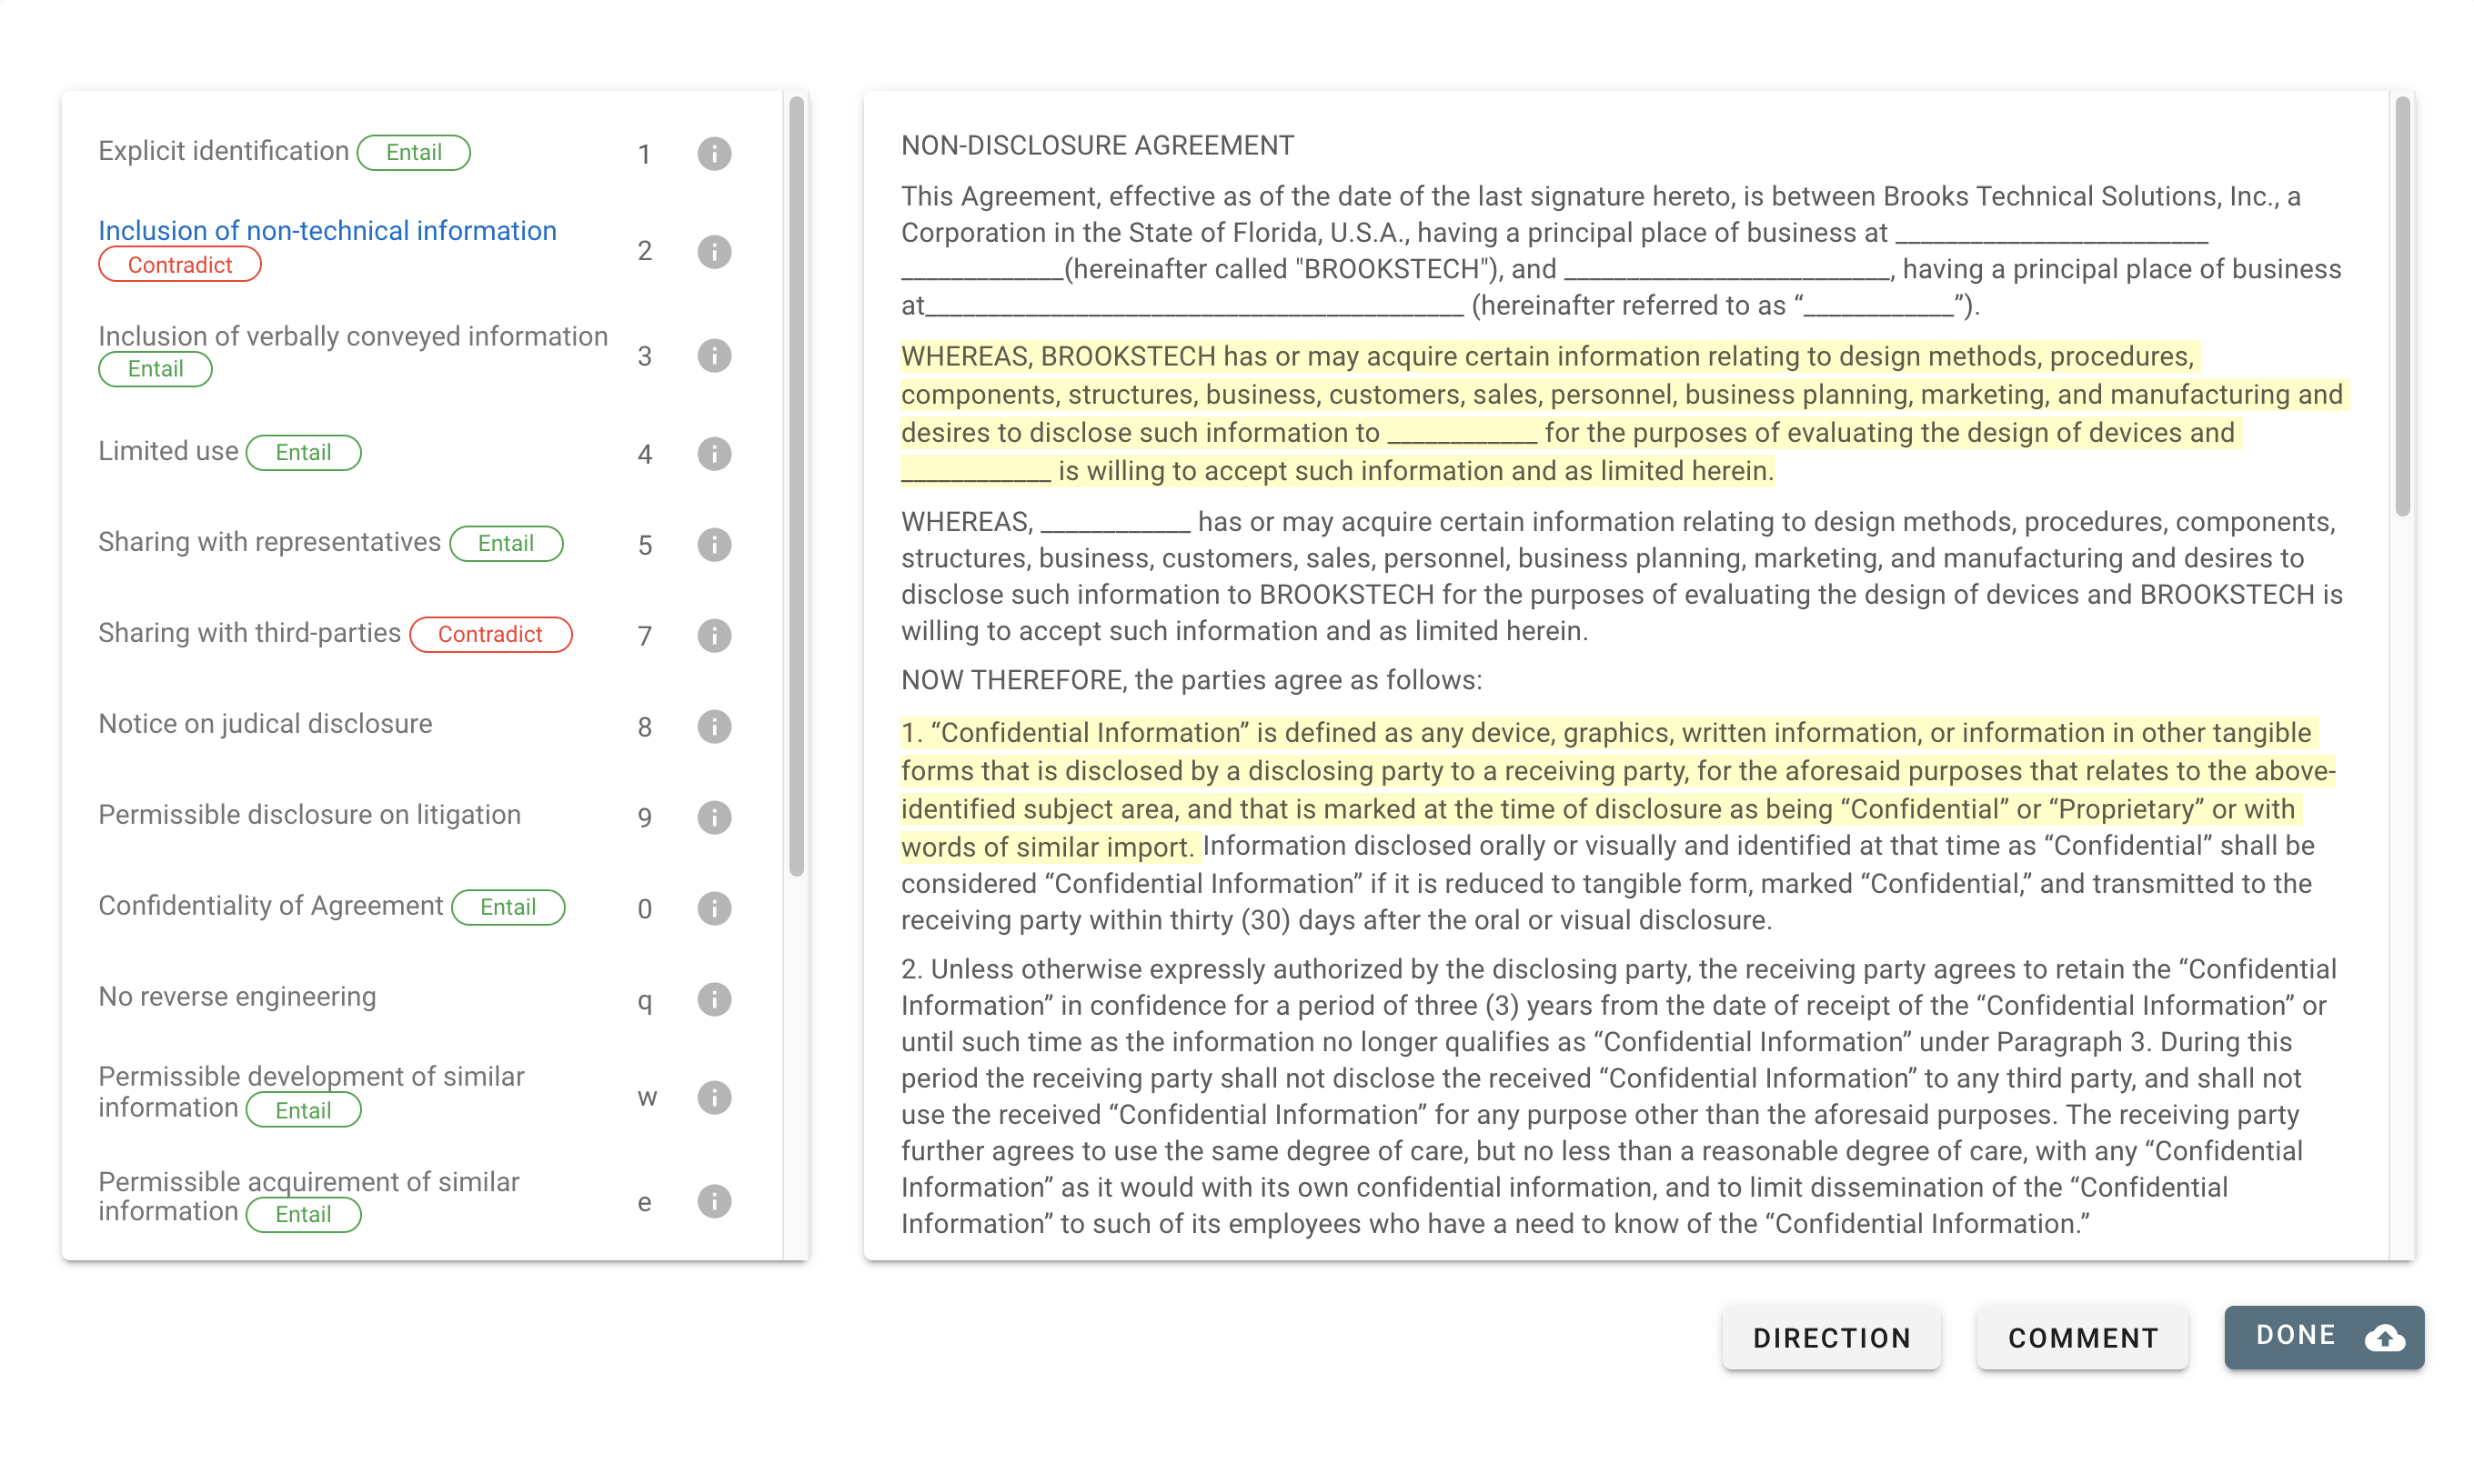
\includegraphics[width=\textwidth]{fig/annotation_ui-span}
        \caption{Evidence identification}
        \label{fig:annotation_ui-span}
    \end{subfigure}
    \begin{subfigure}[b]{0.49\textwidth}
        \centering
        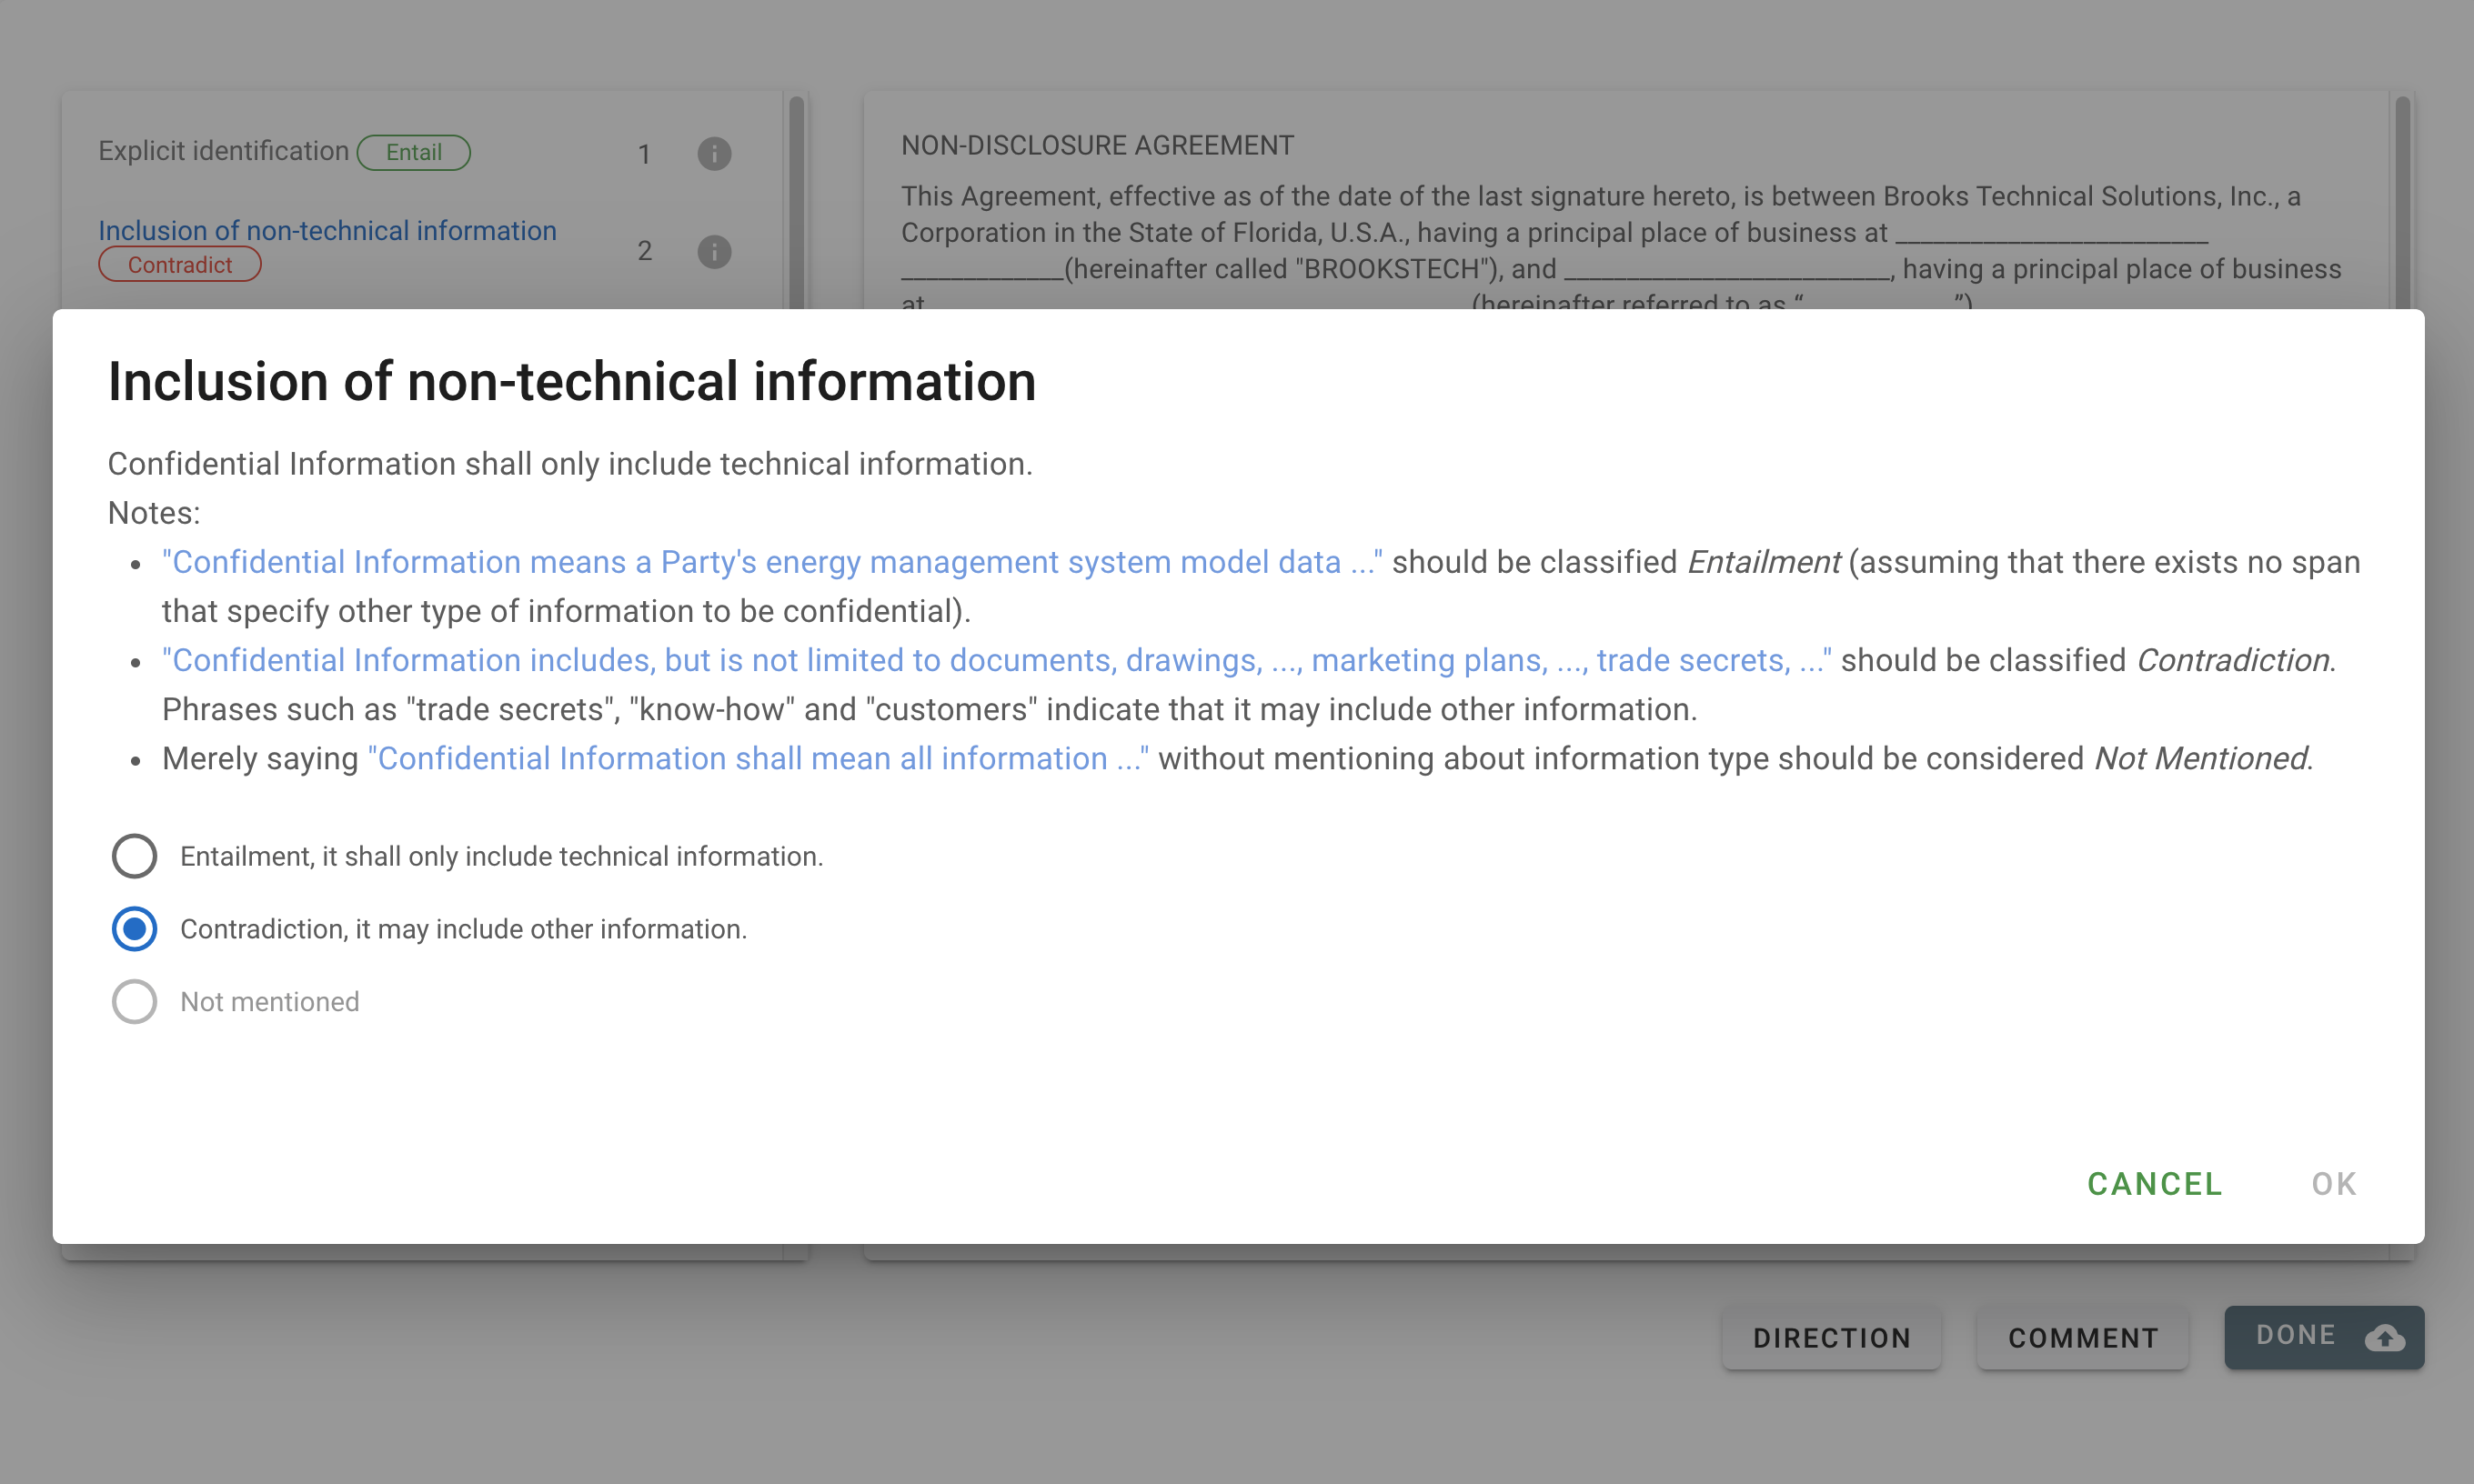
\includegraphics[width=\textwidth]{fig/annotation_ui-nli}
        \caption{NLI}
        \label{fig:annotation_ui-nli}
    \end{subfigure}
    \caption{Question answering with evidence annotation interface}\label{fig:annotation_ui}
\end{figure}

\subsubsection{Details on Contract Annotation}

We developed 17 hypotheses by comparing different NDAs and had them reviewed by paralegals.
List of hypotheses can be found in \cref{tab:hypotheses}.

Since we employ a fixed set of hypotheses unlike existing NLI datasets, we employed an example-oriented annotation guideline for each hypothesis in order to improve annotation consistency.
Furthermore, we developed an annotation interface in order to efficiently and consistently annotate the NDAs.
The interface allows the users to select spans (\cref{fig:annotation_ui-span}) and then a NLI label (\cref{fig:annotation_ui-nli}).

Annotation was conducted by a computational linguistic researcher (the primary annotator) with a help from workers at Amazon Mechanical Turk.
We chose two workers at Amazon Mechanical Turk who were consistently performing well and asked them to redundantly annotate each document with a priority on coverage.
We merged annotated spans for each document.
Finally, the primary annotator reviewed the merged annotations and adjusted the annotations where necessary.
For the train split, the primary annotator only reviewed the annotated spans to judge NLI labels and to consolidate the span boundaries.
For most of the test split, the primary annotator went through the whole contracts to further improve coverage.
Most of the development dataset and some of the test dataset were annotated exclusively by the primary annotator without a help from the workers.
This allowed us to obtain consistent and high coverage annotations.

\subsection{Detailed Experiment Settings}

\subsubsection{Baselines}\label{sec:appendix-experiments-baseline}

We provide supplemental information of the baselines discussed in \cref{sec:baselines}.

For Doc TF-IDF+SVM, Span TF-IDF+Cosine and Span TF-IDF+SVM, we tokenized the input using Stanza \cite{qi-etal-2020-stanza} and extracted unigram TF-IDF vectors using Scikit-learn's \cite{pedregosa_2011} \texttt{TfidfVectorizer} with the default configuration (i.e., no stopwords apart from punctuations, minimum document frequencies of one, and smoothed inverse document frequencies).
For Doc TF-IDF+SVM and Span-TF-IDF+SVM, we used a Support Vector Machine \cite[SVM;][]{chang_libsvm_2011} with a linear kernel with the default hyperparameters implemented in Scikit-learn (i.e., $C=1.0$ with a stopping tolerance of $0.001$).

\begin{table*}[t]
    \centering
    \fontsize{8pt}{10pt}\selectfont
%    \setlength{\tabcolsep}{4pt}
    \renewcommand{\arraystretch}{1.0}
    \begin{tabular}{cccc}\toprule
        Hyperparameter & BERT\textsubscript{\textit{base}} & BERT\textsubscript{\textit{large}} & DeBERTa\textsubscript{\textit{xlarge}} \\\midrule
        Batch size & 32 & 32 & 32  \\
        Learning rate & 1e-5, 2e-5, 3e-5, \textbf{5e-5}  & 1e-5, \textbf{2e-5}, 3e-5, 5e-5 & 5e-6, 8e-6, 9e-6, \textbf{1e-5}  \\
        AdamW's $\epsilon$ & 1e-8 & 1e-8 & 1e-6  \\
        Weight decay & 0.0, \textbf{0.1} & \textbf{0.0}, 0.1 & 0.01  \\
        Max. gradient norm & 1.0 & 1.0 & 1.0  \\
        Warmup steps & 0, \textbf{1000} & 0, \textbf{1000} & \textbf{50}, 100, 500, 1000  \\
        \# epochs & \textbf{3}, 4, 5 & \textbf{3}, 4, 5 & 3, \textbf{4}, 5  \\\midrule
        Min. \# surrounding tokens $n$ & \textbf{64}, 128 & 64, \textbf{128} & \textbf{64}, 128 \\
        Loss weight $\lambda$ & 0.05, 0.1, \textbf{0.2}, 0.4 & \textbf{0.05}, 0.1, 0.2, 0.4 & 0.05, 0.1, 0.2, \textbf{0.4} \\
        Use weighted NLI & \textbf{\texttt{True}}, \texttt{False} & \textbf{\texttt{True}}, \texttt{False} & \textbf{\texttt{True}}, \texttt{False} \\
        \bottomrule
    \end{tabular}
    \caption{Hyperparameter search space. The hyperparameters below the middle line are the hyperparameters specific to Span NLI BERT. The bold values denote the best hyperparameters in our experiment.}\label{tab:hyperparameters}
\end{table*}


For SQuAD BERT, we tried to be as faithful to a commonly used implementation as possible.
Thus, we implemented SQuAD BERT by implementing preprocessing and postprocessing scripts for the Huggingface's implementation\footnote{\url{https://github.com/huggingface/transformers/blob/0c9bae09340dd8c6fdf6aa2ea5637e956efe0f7c/examples/question-answering/run_squad.py}; We have slightly modified their implementation so that we have access to start/end token probabilities.}.
Because the SQuAD BERT only utilizes the first span even if a training example included multiple spans, we created an example for each span of each document-hypothesis pair.
Within the Huggingface's implementation, each example is further split into contexts with a fixed window size.
It is trained to point at starting and ending tokens of the span, or at \texttt{[CLS]} token when a span is not present.
Instead of allowing it to predict spans at arbitrary boundaries, we calculate a score for each of predefined spans by averaging token scores associated with the start and end of the span over different context windows.
This makes sure that its performance is not discounted for getting span boundaries wrong.

\subsubsection{Hyperparameters}\label{sec:appendix-experiments-hyperparameters}

For Span NLI BERT, we ran the same experiment ten times with different hyperparameters (\cref{tab:hyperparameters}).
Hyperparameter search spaces for BERT and DeBERTa have been adopted from \cite{devlin_bert_2019} and \cite{he_deberta_2021}, respectively.
For the SQuAD BERT baseline, we ran hyperparameter search over 18 hyperparameter sets as described in \cite{devlin_bert_2019}.

In both cases, we report the average score of three models with the best development scores.
Since NLI is more challenging than evidence identification, we used macro average NLI accuracy for the criterion.

The choice of weighted/unweighted NLI probablities was a part of our hyperparameters and we found that the best models (for BERT\textsubscript{\textit{base}}, BERT\textsubscript{\textit{large}} and DeBERTa\textsubscript{\textit{xlarge}}) preferred the weighted probablities.
The models with weighted probablities had on average 0.782 (BERT\textsubscript{\textit{base}}) and 0.803 (BERT\textsubscript{\textit{large}}) macro average NLI accuracies whereas the models with unweighted probablities had on average 0.458 (BERT\textsubscript{\textit{base}}) and 0.454 (\textsubscript{\textit{large}}) macro average NLI accuracies.
This implies that it is critical to incorporate the weighted probablities.

As for the loss weight $\lambda$, we found in pilot experiments that NLI starts to overfit faster than span detection, thus we searched values in $\lambda < 1$.
A possible hypothesis is that there is less diversity in teacher signal for NLI than that for evidence span detection; Contexts extracted from a single hypothesis-document pair have the same NLI label which could be somewhat redundant, whereas each context has a different span label.
